\chapter{Podejście low-code/no-code}
Low-Code oraz no-code to nowe podejście skupiające się na umożliwieniu tworzenia programów w sposób nie wymagający znajomości języka oprogramowania. Podejście to ma pozwolić osobom nie będącymi programistami na tworzenie aplikacji biznesowych. Ma to zwiększyć tempo tworzenia rozwiązań biznesowych, na które zapotrzebowanie wciąż rośnie. Jednakże podejście to jest stosounkowo świeżym podejściem, którego początki można było obserwować w codziennym życiu na przykład podczas tworzenia stron internetowych korzystając z narzędzi takich jak \textit{Wordpress}, \textit{Joomla}, \textit{Wix}. Narzędzia te umożliwiają w łatwy sposób tworzyć stronę z tak zwanych kafelków, które umieszczone w odpowiednim miejscu były odpowiedzialne za jedną konkretną rzecz\cite{Wordpress2023, Joomla2023, Wix2023}. Przykład na \refsource{obrazie}{fig:pa-plat}, \textbf{\ref{fig:wp-plat}}.
\begin{figure}[H]
    \centering
    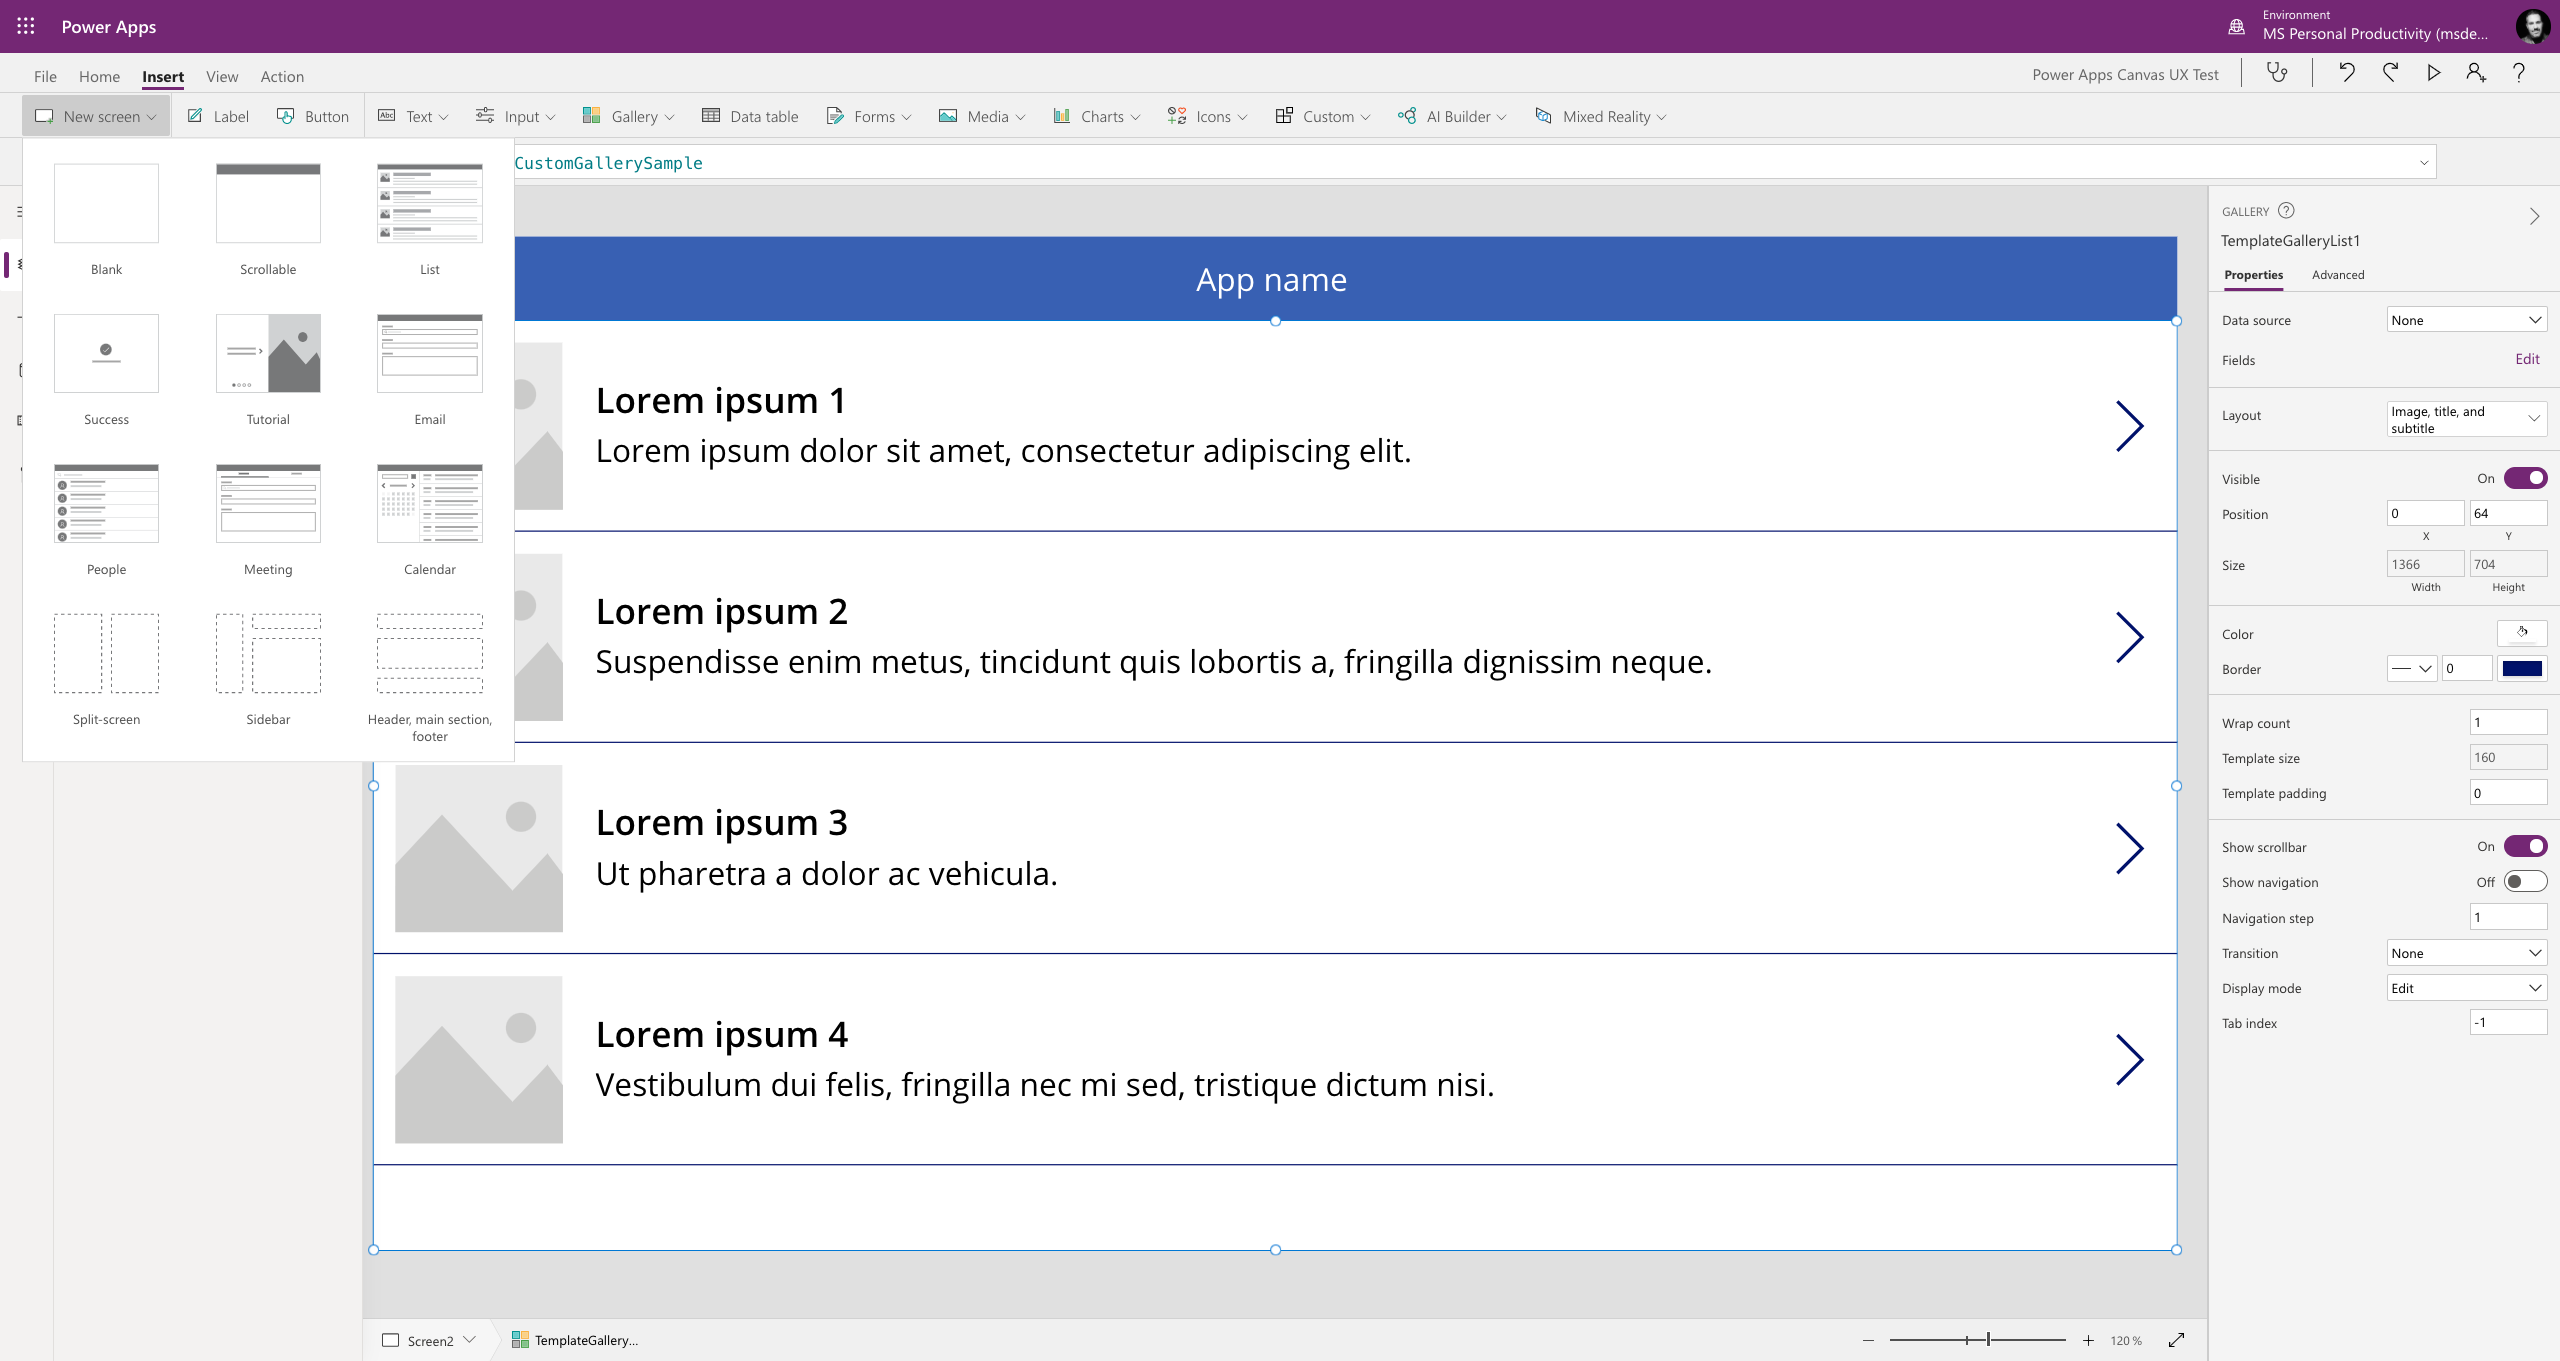
\includegraphics[width=0.6\textwidth]{images/ms_powerapps}
    \captionsource{PowerApps od Microsoft}{\cite{Powerapps2023}}
    \label{fig:pa-plat}
\end{figure}

\begin{figure}[H]
    \centering
    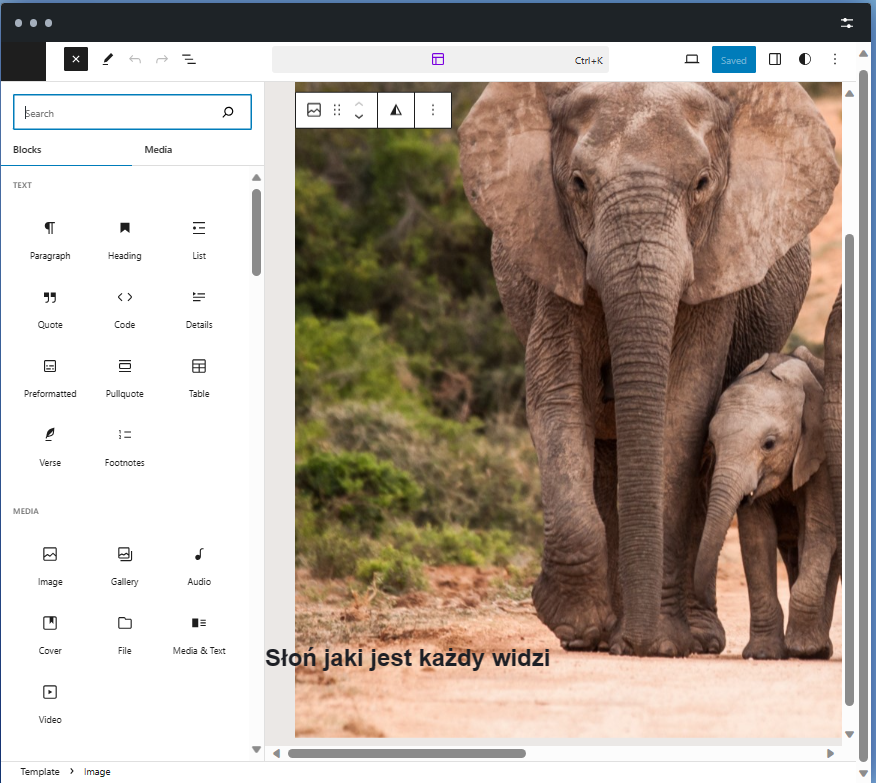
\includegraphics[width=0.4\textwidth]{images/slon_wordpress}
    \captionsource{Wordpress.com}{\cite{WordpressDeveloper2023}}
    \label{fig:wp-plat}
\end{figure}

Coraz większa popularnością cieszą się platformy low-code\trans{ang. Low-code Development Platforms} (\textbf{LCDPs}) dostarczane między innymi przez Google, Microsoft, Amazon pozwalają one na tworzenie wysoko skalowalnych rozwiązań przy niewielkim albo i żadnym nakładzie programowania. Ma to umożliwić osobom z niewielkim doświadczeniem w programowaniu, na szybkie wdrożenie oraz tworzenie niezawodnego oprogramowania. Twórcy platform oferują również korzystającym zmniejszenie ilości pracy potrzebnej do wdrożenia albo rozwijania kolejnych funkcjonalności\cite{Bock2021, Hirzel2022}.
\\ \\
\section{Platformy}
LCDP udostępniane twórcom aplikacji, umożliwiają skalowalność rozwiązań tworzonych na własne potrzeby. Dodatkowo są popularne przy tworzeniu aplikacji typu ''\textit{aplikacja jako usługa}'' \trans{ang. Software-as-a-Service} (SaaS), które opłacane są tylko za stopień ich użycia, co w niektórych przypadkach może się okazać dużo bardziej opłacalne niż utrzymywanie swoich rozwiązań serwerowych. Dzięki takim rozwiązaniom wiele małych firm będzie mogło pozwolić sobie na tworzenie i utrzymywanie dostosowanych rozwiązań opartych o ekosytem \textit{Microsoft365} / \textit{Google Workspace}.

\subsection{Microsoft PowerApps}
Jest to platforma programistyczna umożliwiająca tworzenie niestandardowych aplikacji dla rozwiązań biznesowych. Umożliwia ona tworzenie aplikacji opartych o różnorakie źródła danych do których należą między innymi: SQL Server, SharePoint, Dynamics 365. Dodatkową zaletą tego rozwiązania jest tworzenie aplikacji responsywnych, działających dobrze na wielu rodzajach urządzeń. Dodatkowow platforma ta pozwala tworzyć trzy typy aplikacji przy braku konieczności kodowania\cite{Microsoftc}
\begin{itemize}
    \item \textbf{Kanwa} - jest to typ aplikacji oparty o model danych znajdujący się na przykład w Excelu. Aplikację tego typu tworzy się za pomcą przesuwanych kafelek, a proces przypomina po trochu robienie prezentacji przy użyciu aplikacji Powerpoint, co umożliwia pełną dowolność w tworzonym interfejsie graficznym\cite{Microsoftb}.

    \item \textbf{Oparte na modelu} - w ramach korzystania z usługi Microsoft Dataverse można wygenerować aplikacje bazujące na danym modelu danych, przez co użytkownicy otrzymują produkt ułatwiający im analizę danych\cite{Microsofta}.

    \item \textbf{Karty} - są to uproszczone aplikacje, które można dodać do usługi Micrsoft Teams w określonym biznesowym celu. Dużą zaletą tego rozwiązania jest możliwość korzystania z źródeł danych, dzięki czemu poszczególne karty mogą odpowiadać za jedno zadanie biznesowe\cite{Microsoft}.
\end{itemize}

\subsection{Amazon QuickSight}
Jest to rozwiązanie firmy Amazon, które umożliwia firmom dostarczanie rozwiązań z zakresu analityki biznesowe\trans{ang. business intelligence} (BI) dzięki interaktywnym pulpitom korzystającym z jednego źródła prawdy. Dodatkowo korzystanie z interaktywnych formularzy, raportów oraz zapytań w języku naturalnym pozwala interesariuszom otrzymać możliwość korzystania z jednolitych rozwiązań opartych o różne modele danych\cite{AmazonQuickSight}.

\subsection{Google AppSheet}
Platforma AppSheet od firmy Google umożliwia tworzenie aplikacji mobilnych oraz desktopowych bez użycia kodu. Firma wskazuje na możliwości integracyjne z różnymi dostawcami danych, do których należą między innymi Microsoft, Dropbox, a także wbudowaną integrację z aplikacjiami Google Workspace do któych należą Gmail, Sheets oraz Spaces. Platforma pozwala również na tworzenie automatycznych botów, które wykonują zadania w oparciu o bodźce zewnętrzne bądź wewnętrzne. Narzędzie pozwala w prosty sposób na tworzenie szybkich rozwiązań biznesowych w oparciu o ekosystem firmy Google\cite{GoogleAppSheet}.


